% *** DOCUMENT CLASS ***%
\documentclass[11pt,compress]{beamer} % handout,
\usetheme{Madrid}
\usecolortheme{crane}
\useoutertheme[subsection=false,shadow]{miniframes}

% ! full class documentation available here
% http://tug.ctan.org/macros/latex/contrib/beamer/doc/beameruserguide.pdf

%===============================================
% *** GENERAL PACKAGES *** %
\usepackage[utf8]{inputenc}
\usepackage[english]{babel}
\usepackage{csquotes}
\usepackage{array}
\usepackage{booktabs}
\usepackage{multirow}
\usepackage{color}
\usepackage{lipsum}

%===============================================
% *** ALGORITHM PACKAGE *** %
\usepackage[ruled,vlined]{algorithm2e}
\newcommand{\forcond}[2]{#1 \KwTo #2}
\SetAlgoSkip{}

%===============================================
% *** GRAPHICS RELATED PACKAGES *** %
\usepackage{graphicx}
\DeclareGraphicsExtensions{.pdf,.jpg,.png,.gif}
\graphicspath{img}

%===============================================
% *** MATH PACKAGES *** %
\usepackage{amsfonts}
\usepackage{amsmath}
\usepackage{amsthm}
\usepackage{amssymb}
\usepackage{mathrsfs} % Ralph Smith’s Formal Script Font : mathrsfs{A}
\usepackage{mathtools}
\usepackage{siunitx}  % physics units
\usepackage{bm}
\usepackage{stmaryrd}

%===============================================
% *** BIBLIOGRAPHY PACKAGE *** 
\usepackage[backend=biber, style=authortitle]{biblatex}
\addbibresource{_report.bib}
\usepackage{appendixnumberbeamer}

% display table of content at the beginning of each section
\AtBeginSection[] {
    \ifnum \value{section}=1
      {
      \begin{frame}
        \frametitle{Overview}
          \small \tableofcontents[sectionstyle=show/shaded]
      \end{frame}
      }
    \else{
      \begin{frame}
          \small \tableofcontents[currentsection,sectionstyle=show/shaded,hideothersubsections]
      \end{frame}}
    \fi
    }
   \setbeamertemplate{caption}[numbered]
   
   \newcommand\blfootnote[1]{%
    \begingroup
    \renewcommand\thefootnote{}\footnote[frame]{#1}%
    \addtocounter{footnote}{-1}%
    \endgroup
   }

\begin{document}

\title[]{Detection of AI-generated images}
\author{Lucas SALAND\\ Supervisor: Patrick Bas}
\institute{Université de Lille}
\date[\today]{
\includegraphics[keepaspectratio,width=0.2\textwidth]{img/cristal.png} \medskip \\ Lille, France \medskip \\ \today}

\frame{\titlepage}

\section*{Overview}
\begin{frame}
  \tableofcontents
\end{frame}

\section{AI image generation}
\subsection{GAN}
\begin{frame}{GAN}
  \begin{figure}
    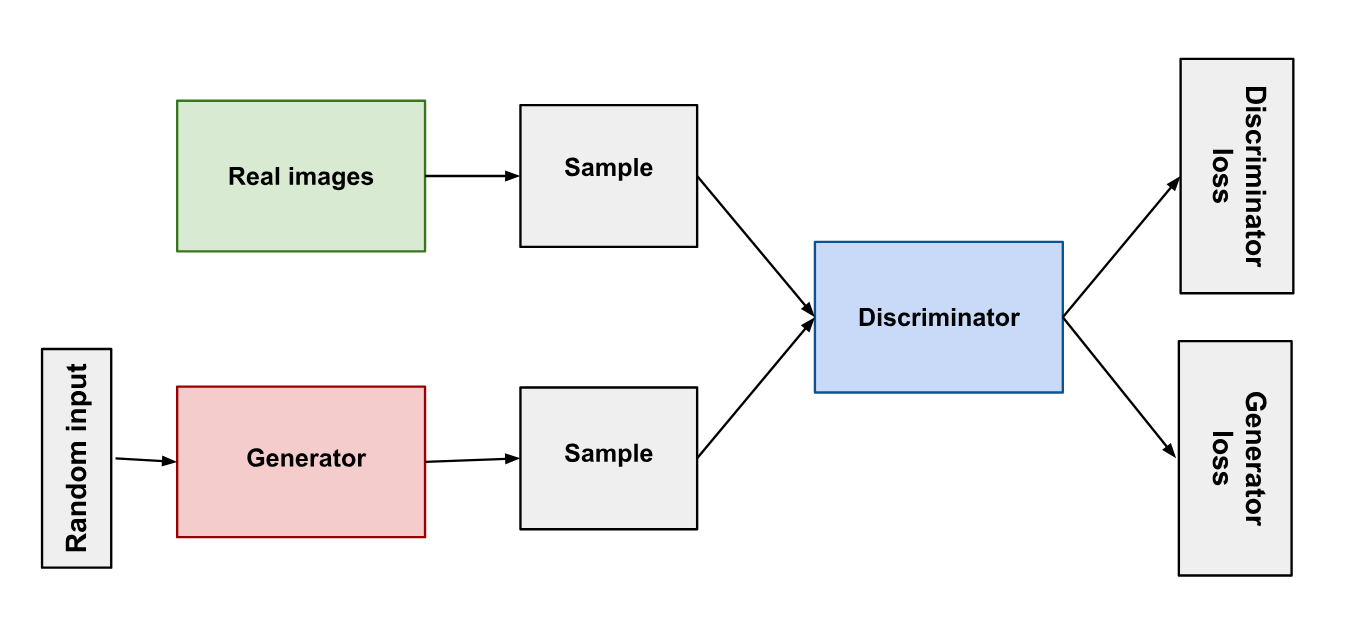
\includegraphics[width=\textwidth]{img/GAN.png}
  \end{figure}
\end{frame}

\subsection{Diffusion model}
\begin{frame}{Diffusion model}
  \begin{figure}
    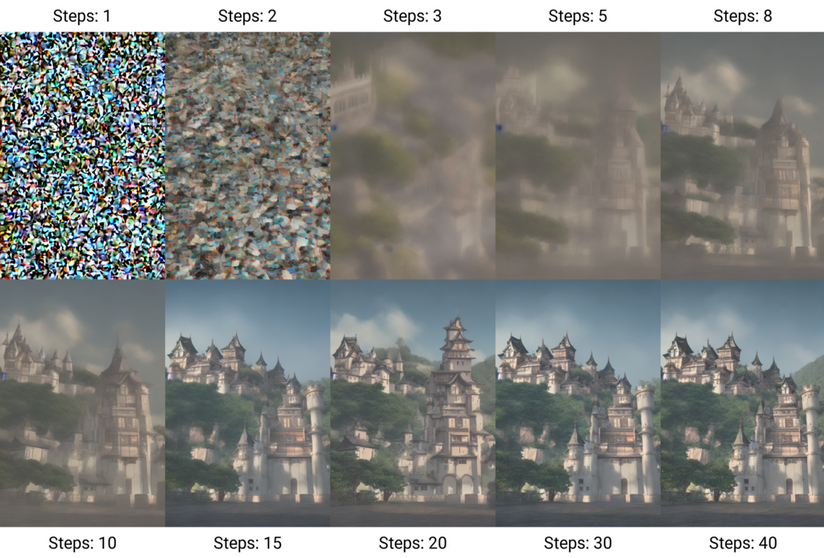
\includegraphics[width=.8\textwidth]{img/diffusion.png}
  \end{figure}
\end{frame}

\section{AI-generated images detection}
\subsection{CLIP}
\begin{frame}
    \frametitle{CLIP}
    \begin{figure}
        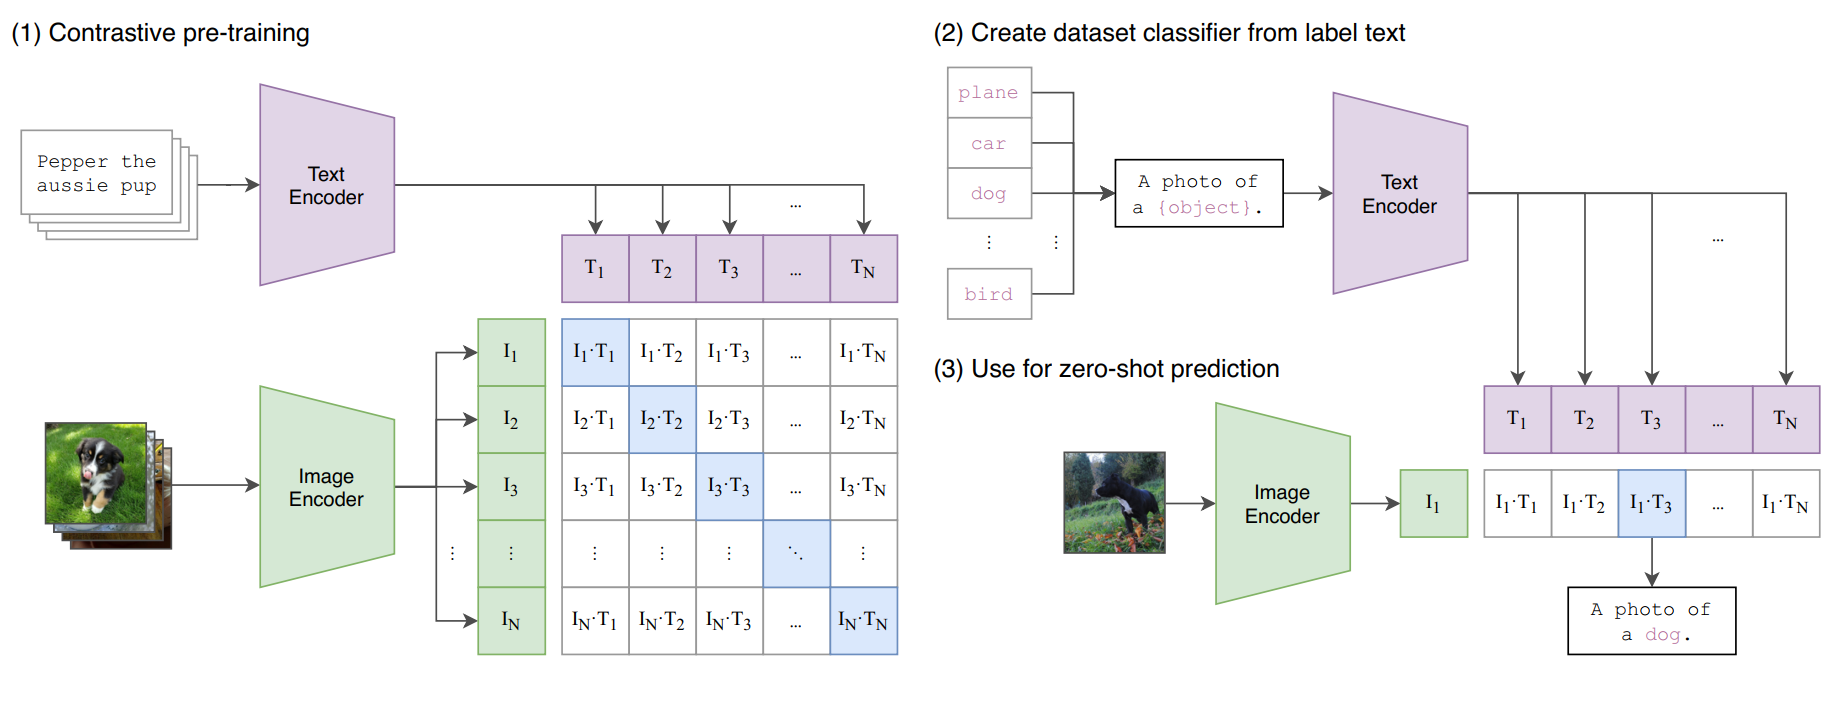
\includegraphics[width=\textwidth]{img/CLIP.png}
    \end{figure}
\end{frame}

\begin{frame}
  \frametitle{CLIP for detection}
  \only<1-4>{
    Method proposed in \autocite*{cozzolinoRaisingBarAIgenerated2024}:
  \begin{itemize}
    \pause
    \item Build a dataset of pairs of real and generated images
    \pause
    \item Extract the CLIP features
    \pause
    \item Train a SVM on these features
  \end{itemize}}
\end{frame}

\begin{frame}
  \frametitle{ELSA dataset}
  \begin{figure}
    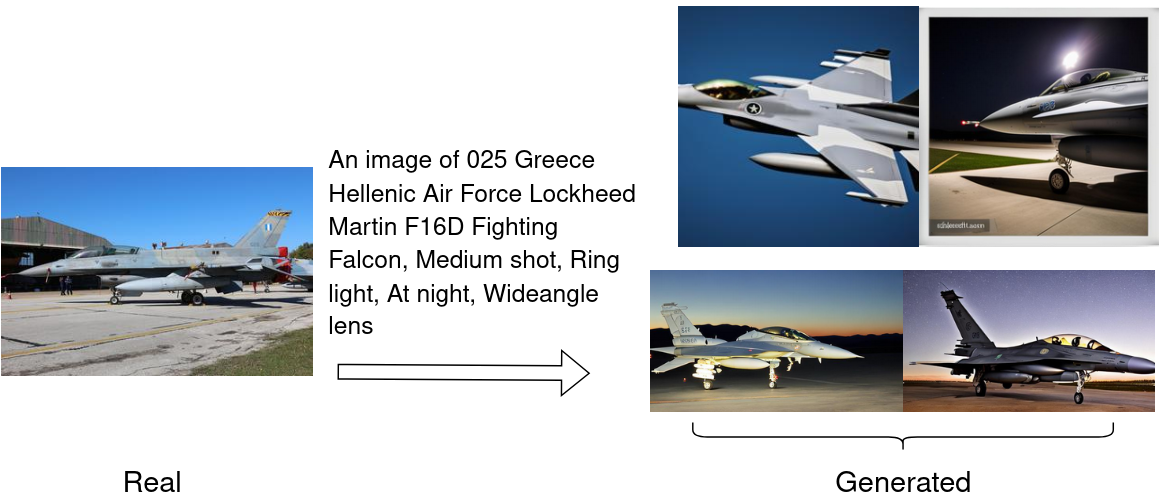
\includegraphics[width=\textwidth]{img/ELSA.png}
  \end{figure}

\end{frame}

\subsection{Impact of JPEG compression}
\begin{frame}
    \frametitle{JPEG compression's impact}
    \only<1>{
    \begin{figure}
        \includegraphics[width=\textwidth]{img/jpeg.png}
    \end{figure}
    }
    \only<2>{
    \begin{table}[H]
        \centering
        \begin{tabular}{|c|c|c|c|c|}
        \hline
        & \multicolumn{4}{c|}{Test} \\
        \cline{2-5}
         & quality & 40 & 65 & 90 \\
        \hline
        \multirow{3}{*}{Train} & 40 & 0.9813 & 0.9730 & 0.9797 \\
         \cline{2-5}
         & 65 & 0.9450 & 0.9825 & 0.9830 \\
         \cline{2-5}
         & 90 & 0.7744 & 0.8581 & 0.9925 \\
        \hline
        \end{tabular}
        \caption{Accuracy of binary classification for pairs of qualtity factors for train and test.}
        \label{table:jpeg}
    \end{table}
    }
\end{frame}


\subsection{Generators diversity and neural network}
\begin{frame}{Generators diversity and neural network}
  \begin{columns}
    \begin{column}{.4\textwidth}
      Synthbuster:
      \begin{itemize}
        \item 9 generators
        \item 1000 images per generator
      \end{itemize}
    \end{column}

    \begin{column}{.6\textwidth}
      \begin{figure}
        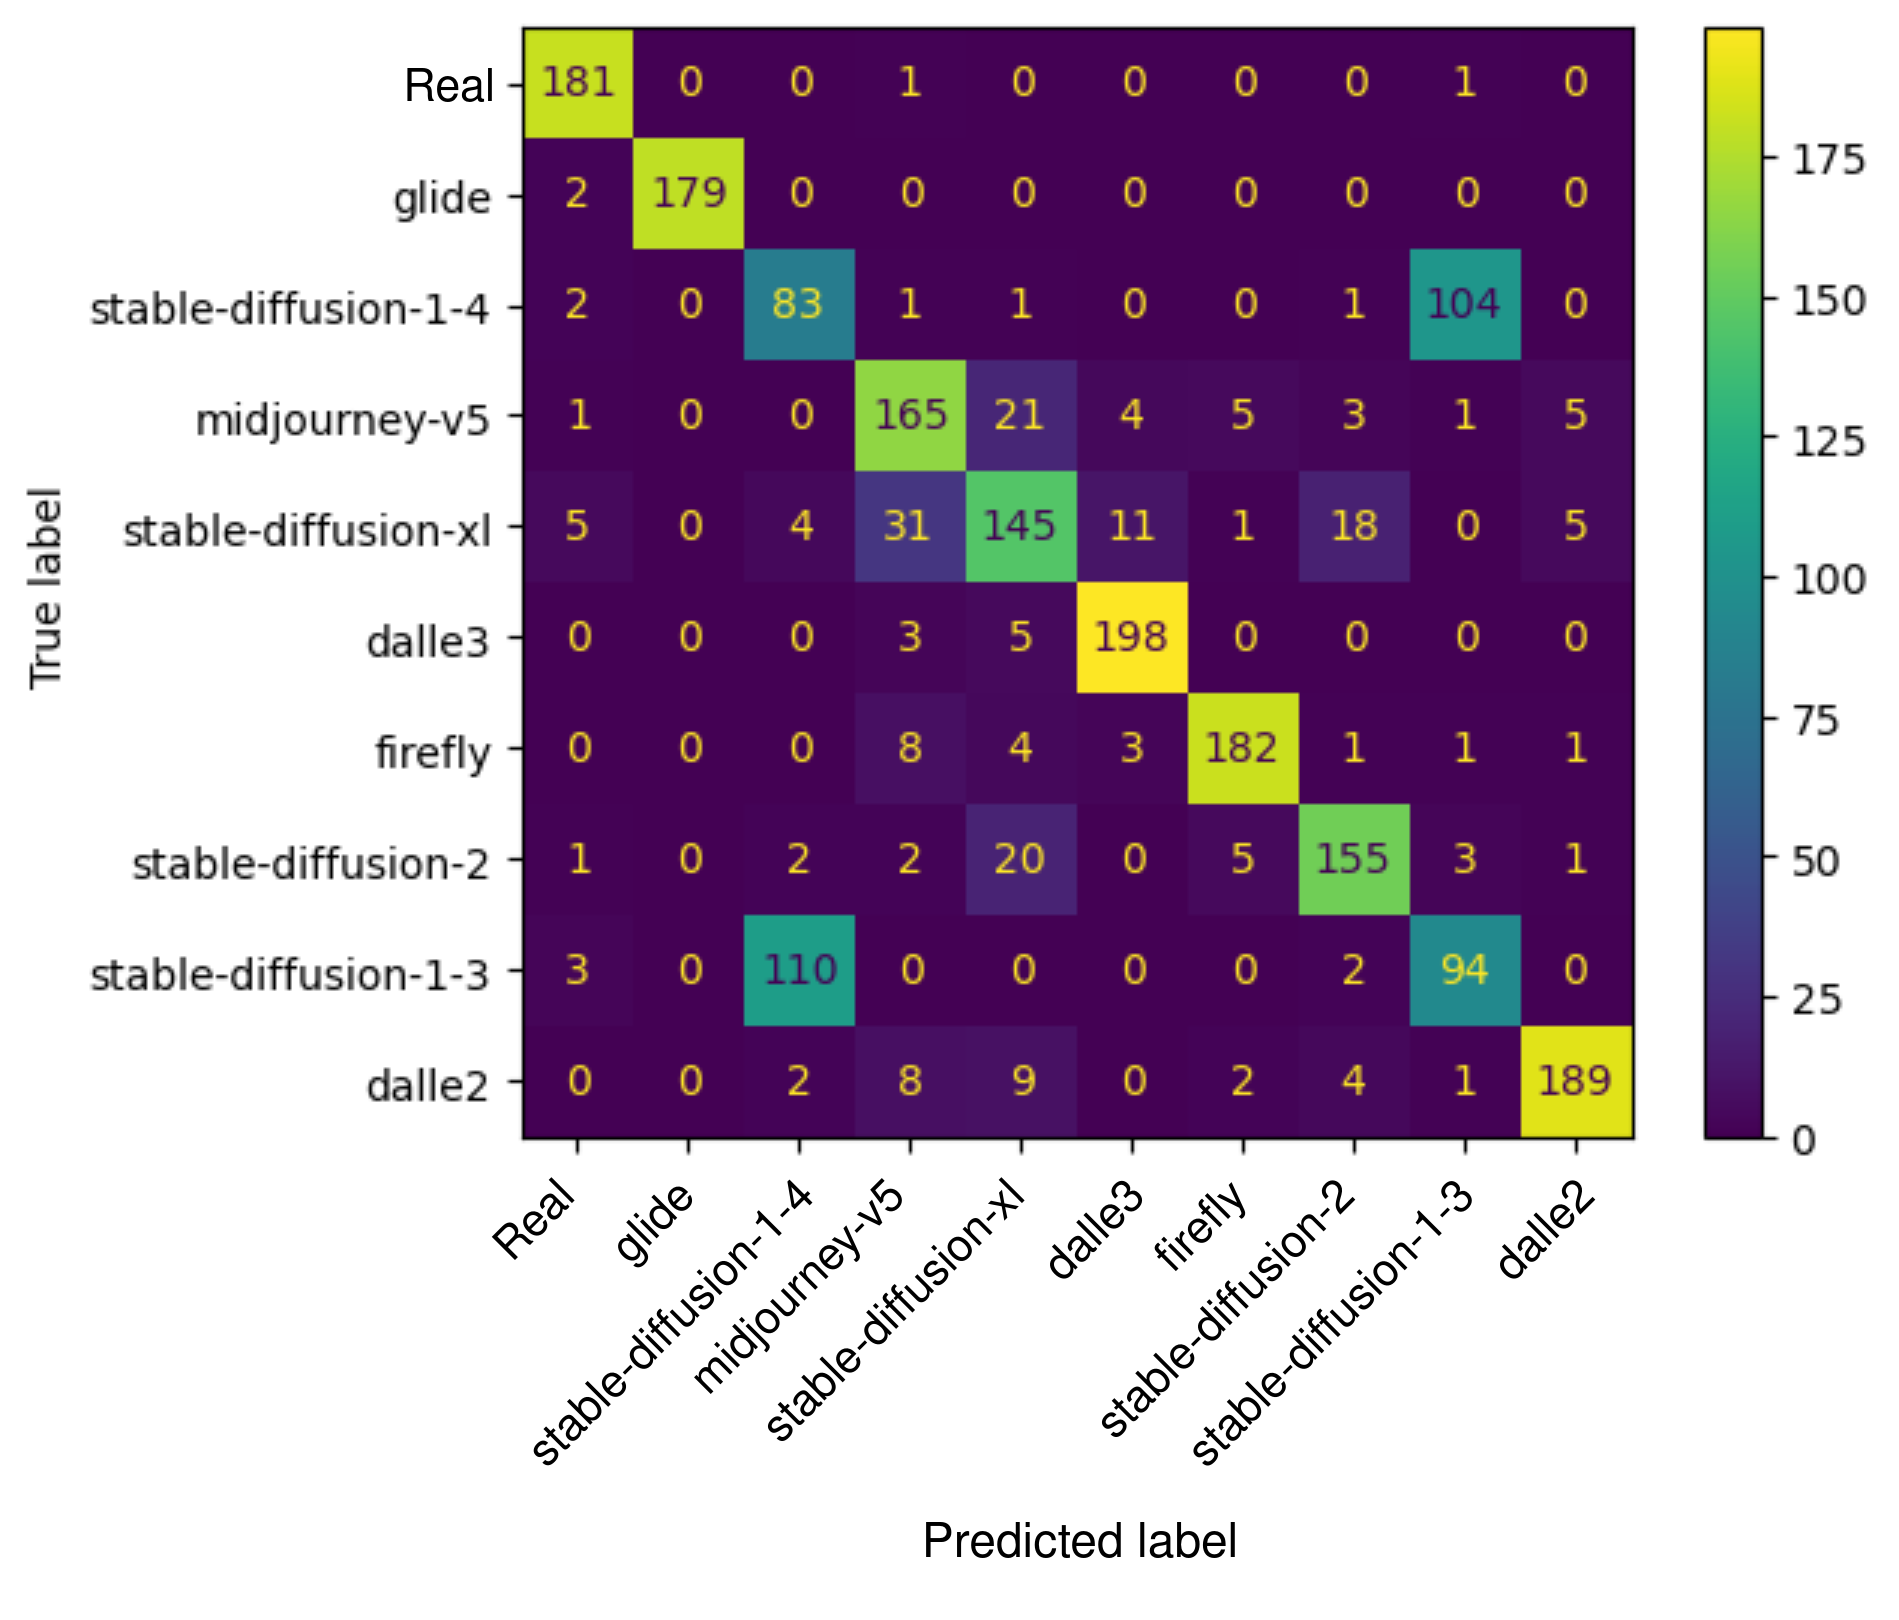
\includegraphics[width=\textwidth]{img/confusion.png}
        \caption{Confusion matrix for a SVM multiclass-classifier trained and tested on synth-
        buster.}
      \end{figure}
    \end{column}
  \end{columns}
\end{frame}

\begin{frame}{Generators diversity and neural network}
  Multi-class classifier for binary classification:
  \begin{figure}
    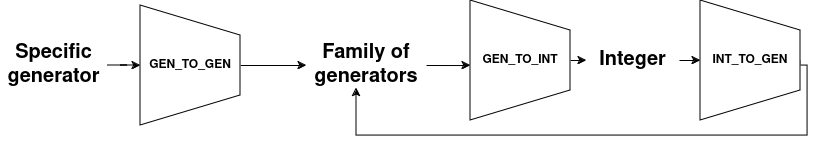
\includegraphics[width=\textwidth]{img/maps.png}
  \end{figure}
\end{frame}

\begin{frame}{SVM vs neural network}
  \begin{table}[H]
    \centering
    \begin{tabular}{|c|p{.3\textwidth}|p{.3\textwidth}|}
        \hline
        Model & Binary classification accuracy & Multi-class classification Accuracy\\
        \hline
        SVM & 0.970 & 0.873\\
        \hline
        Neural network & \textbf{0.974} & \textbf{0.878}\\
        \hline
    \end{tabular}
    \caption{Comparison between SVM and neural network for accuracy in classification task.}
    \label{table:svmVsNN}
  \end{table}
  
  \pause
  \begin{columns}
    \begin{column}{.4\textwidth}
      \begin{itemize}
        \item Code of the detector in a single file
        \pause
        \item Use Pytorch's dataset library
      \end{itemize}
    \end{column}
    \pause
    \begin{column}{.05\textwidth}
      \Huge
      $\Rightarrow$
    \end{column}

    \begin{column}{.4\textwidth}
      Accelerate development
    \end{column}
  \end{columns}
\end{frame}

\begin{frame}{Multi-class classifier for binary detection vs binary classifier}
  The issue: GEN\_TO\_GEN map needs to be updated frequently\\
  \vspace*{.5cm}
  \begin{columns}
    \begin{column}{.5\textwidth}
      Binary detector accuracy: \textbf{0.71}\\
      Multi-class binary accuracy: \textbf{0.73} 
    \end{column}

    \begin{column}{.05\textwidth}
      \huge
      $\Rightarrow$
    \end{column}

    \begin{column}{.4\textwidth}
      Drop the multi-class classifier to accelerate development.
    \end{column}
  \end{columns}
\end{frame}

\begin{frame}{Cleaning the data}
  \centering
  Repetitivity in the semantic of generated images $\rightarrow$ removed generators with repetitivity.
  \begin{figure}[H]
    \centering
    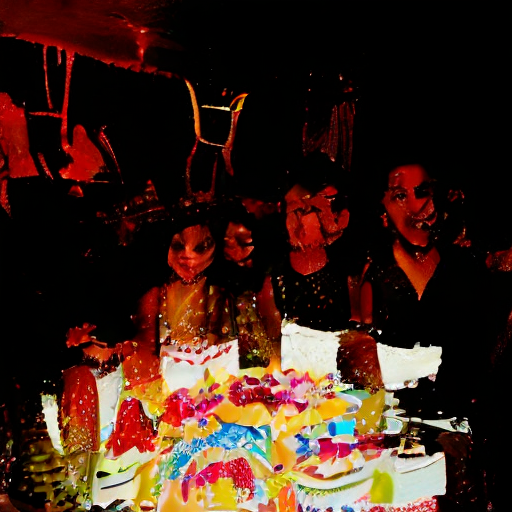
\includegraphics[width=.4\textwidth]{img/birthday1.png}
    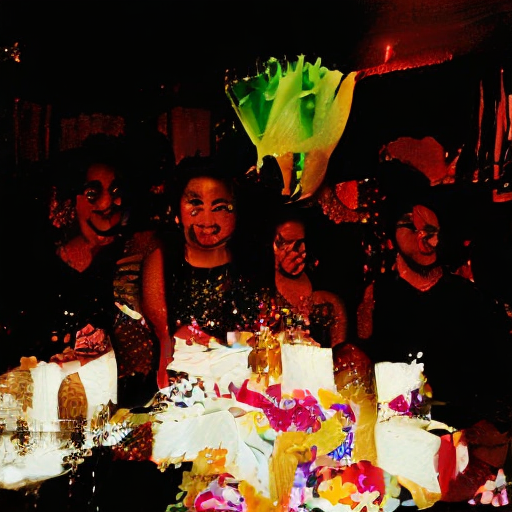
\includegraphics[width=.4\textwidth]{img/birthday2.png}
    \caption{Example of repetition in the content of images. The images are not the same but their semantic is very similar.}
    \label{fig:repetition}
  \end{figure}
\end{frame}

\subsection{Pair training and fine-tuning}
\begin{frame}{Pair training and fine-tuning}
  Pair dataset: 1000 pairs of real and generated images + 1000 generated images from AID and 1000 real images from Flickr.\\
  test\_meta: Real images from Flickr and generated images from 19 generators.
  \begin{table}[H]
    \centering
    \begin{tabular}{|c|c|}
        \hline
        accuracy on OOD before fine-tuning on test\_meta & 0.83 \\
        \hline
        accuracy on OOD after fine-tuning on test\_meta & 0.91 \\
        \hline
        accuracy on test meta before fine-tuning on test\_meta & 0.79 \\
        \hline
        accuracy on test meta after fine-tuning on test\_meta & 0.97 \\
        \hline
    \end{tabular}
    \caption{Accuracy comparison before and after fine-tuning.}
    \label{tab:fine-tuning}
\end{table}
\end{frame}

% \subsection{DoubleCLIP: Another approach to work with pairs}

\subsection{Tip-Adapter}
\begin{frame}{Tip-Adapter}
  \begin{figure}
    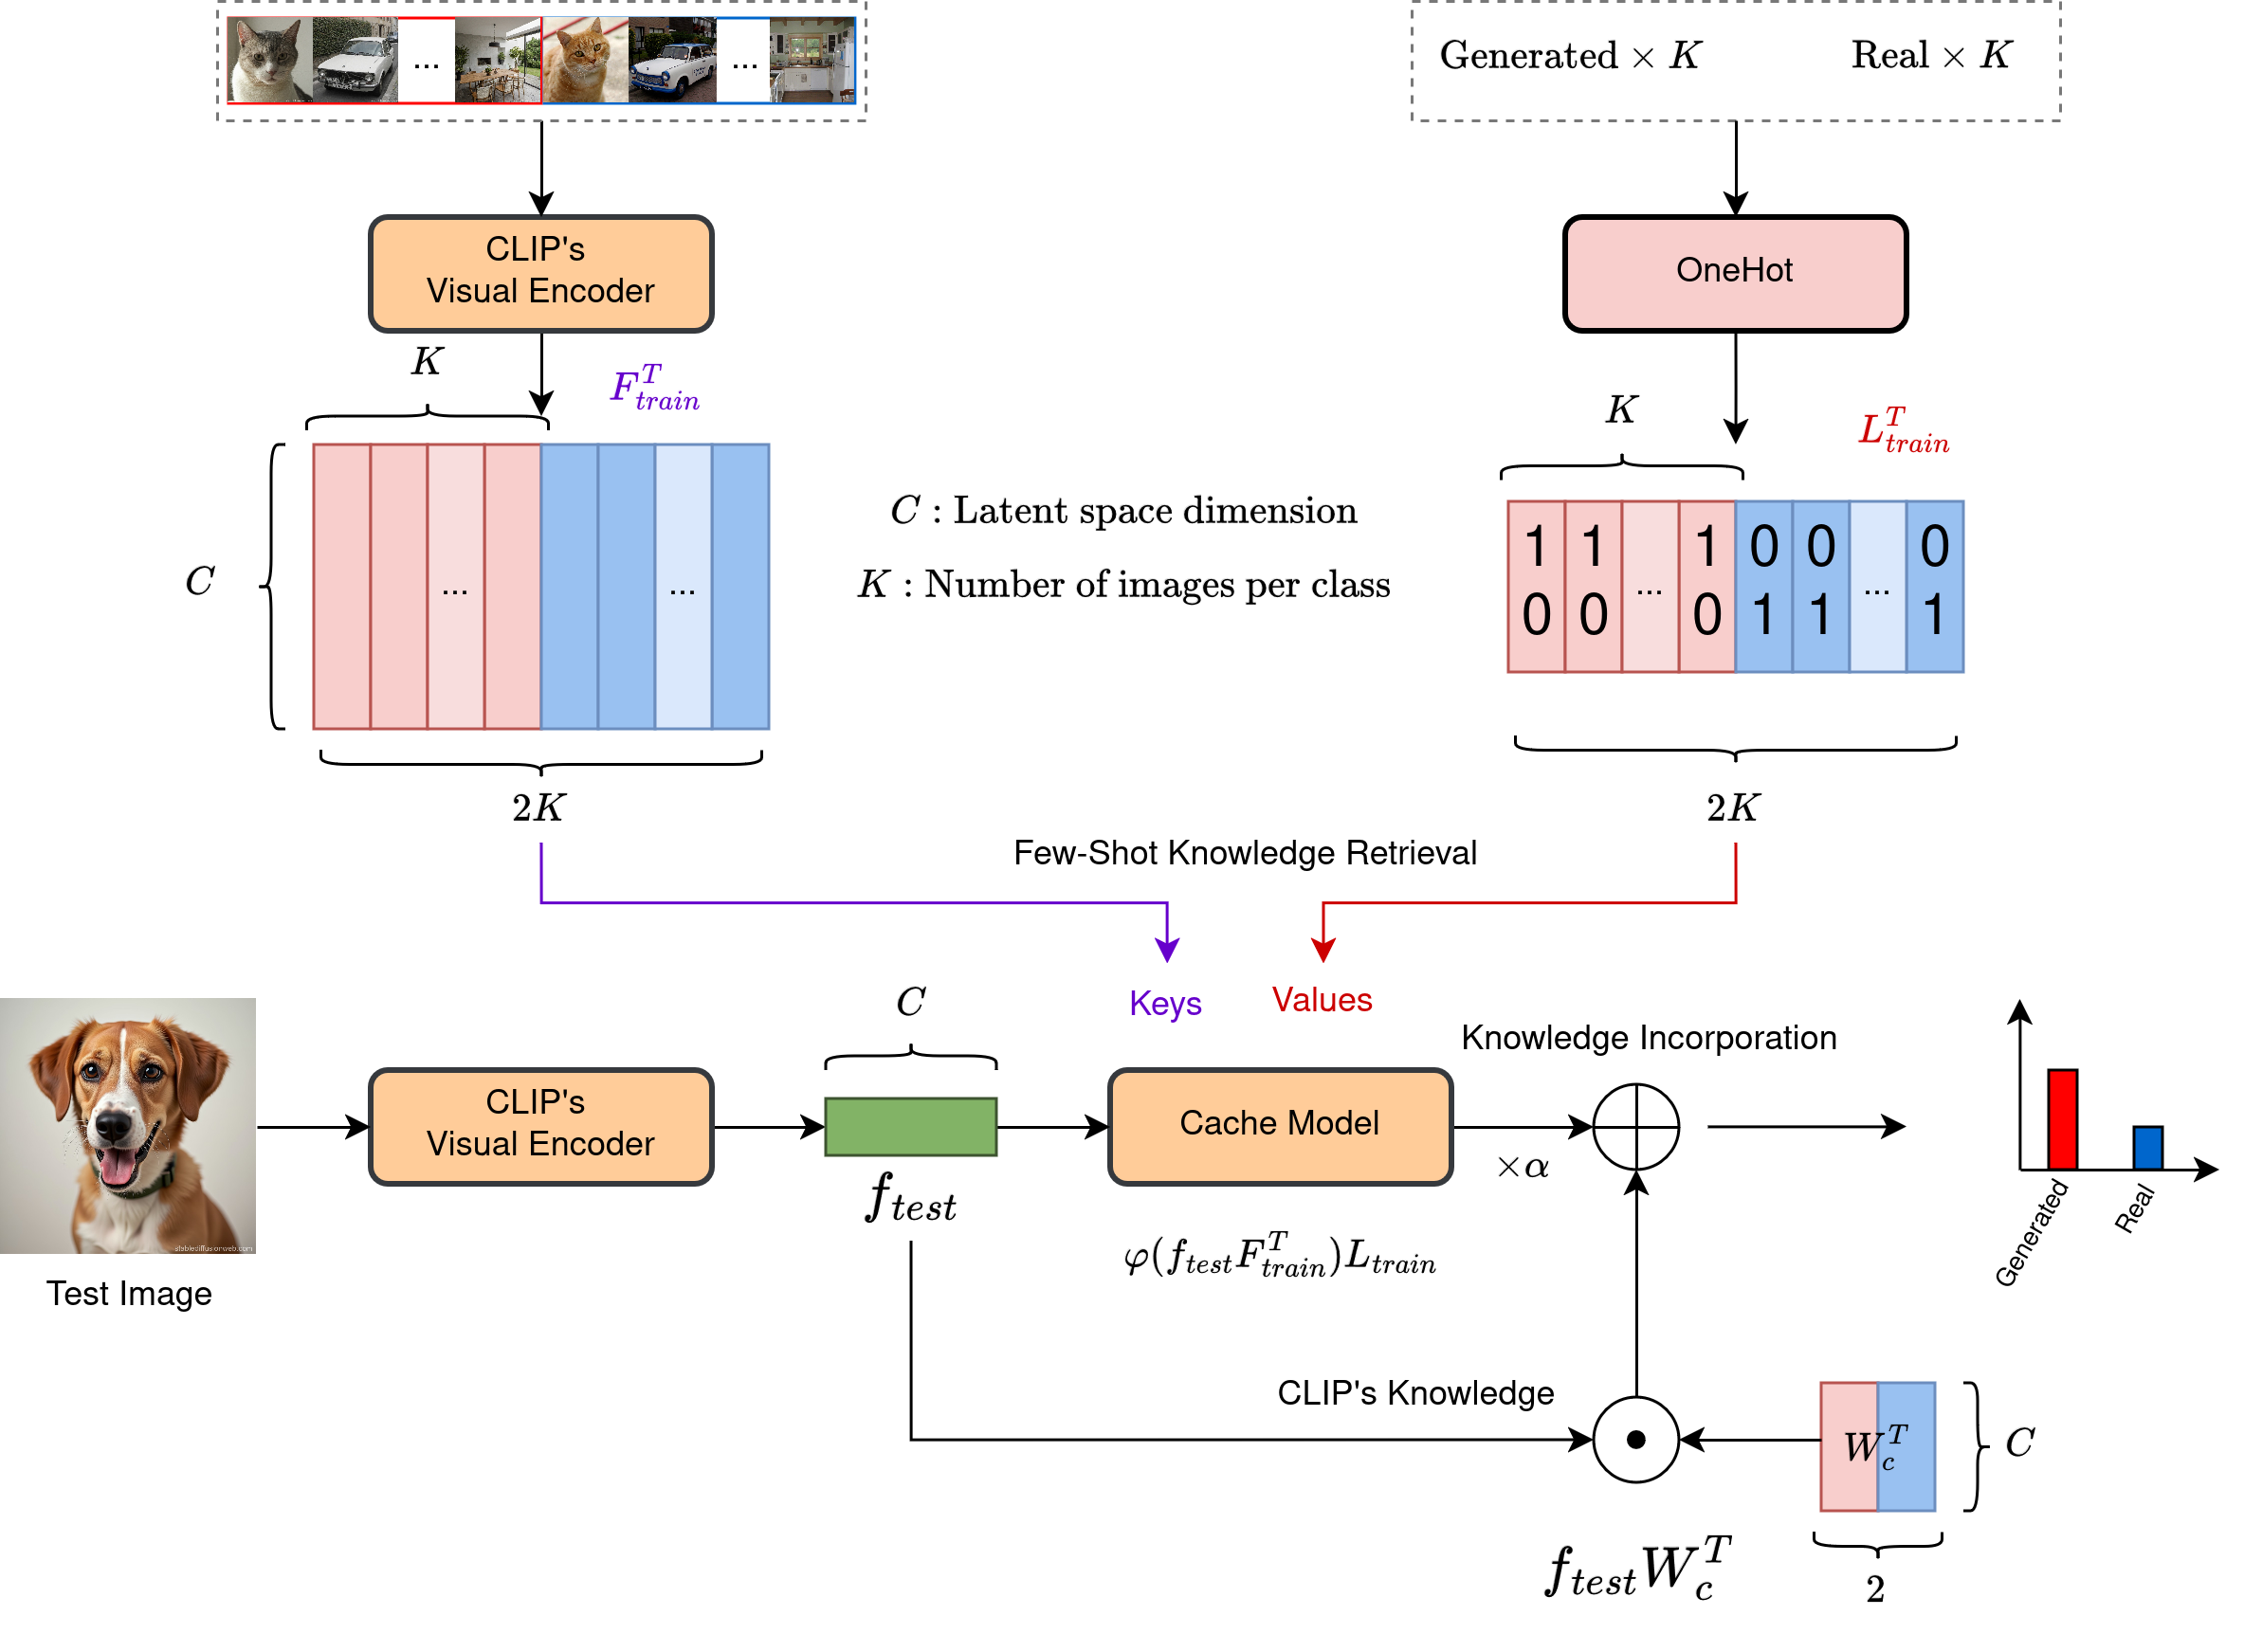
\includegraphics[height=.7\textheight]{img/tip_adapter_binary.png}
  \end{figure}
  \begin{equation}
    logits = \alpha\underbrace{\varphi(f_{test}F_{train}^T)L_{train}}_{\text{Few-shot knowledge}} + \underbrace{f_{test}W_c^T}_{\text{prior knowledge of pretrained CLIP}} \nonumber
  \end{equation}
\end{frame}

\begin{frame}{Tip-Adapter}
    \begin{table}[H]
      \centering
      \begin{tabular}{|c|c|c|}
      \hline
      \textbf{Cache Size} & \textbf{Accuracy on TaskA} & \textbf{Accuracy on test\_meta} \\ \hline
      2    & 0.68 & 0.65 \\ \hline
      4    & 0.69 & 0.71 \\ \hline
      6    & 0.70 & 0.74 \\ \hline
      8    & 0.75 & 0.74 \\ \hline
      16   & 0.72 & 0.77 \\ \hline
      32   & 0.69 & 0.75 \\ \hline
      64   & 0.60 & 0.71 \\ \hline
      128  & 0.70 & 0.76 \\ \hline
      200  & 0.68 & 0.76 \\ \hline
      1000 & 0.69 & 0.75 \\ \hline
      2000 & 0.68 & 0.75 \\ \hline
      \end{tabular}
      \label{tab:cache}
    \end{table}  
  \end{frame}

  \begin{frame}{Tip-Adapter}
    \begin{table}[H]
      \centering
      \begin{tabular}{|c|c|c|}
      \hline
      \textbf{Alpha} & \textbf{Accuracy on TaskA} & \textbf{Accuracy on test\_meta} \\ \hline
      0 & 0.65 & 0.47 \\ \hline
      1 & 0.74 & 0.65 \\ \hline
      2 & 0.75 & 0.71 \\ \hline
      3 & 0.76 & 0.73 \\ \hline
      4 & 0.75 & 0.74 \\ \hline
      5 & 0.75 & 0.74 \\ \hline
      \end{tabular}
      \label{tab:alpha}
    \end{table}  
\end{frame}

\begin{frame}{Tip-Adapter-F}
  \centering
  \begin{figure}
    \includegraphics[width=.7\textwidth]{img/tip_adapter_f_binary.png}
  \end{figure}
\end{frame}

\begin{frame}{Tip-Adapter-F}
  \begin{table}[H]
    \centering
    \begin{tabular}{|c|c|}
    \hline
    \textbf{Number of epochs} & \textbf{Accuracy on taskA} \\ \hline
    5   & 0.85 \\ \hline
    10  & 0.86 \\ \hline
    20  & 0.88 \\ \hline
    50  & 0.89 \\ \hline
    100 & 0.90 \\ \hline
    \end{tabular}
  \end{table}
\end{frame}

\section{Conclusion}
\begin{frame}{Conclusion}
  \begin{itemize}
    \pause
    \item Importance of the diversity of data
    \pause
    \item More experiments on Tip-Adapter-F
    \pause
    \item Good performances despite poor semantic content in images from AID
    \pause
    \item Need to understand CLIP features $\rightarrow$ adversarial attack
  \end{itemize}
\end{frame}
\end{document}